\documentclass[10pt]{article}
\usepackage{commands}
\usepackage{slashed}
% \usepackage{pxfonts}
\pgfplotsset{compat=1.18}
\newcommand{\ddpd}[2]{\frac{\partial #1}{\partial #2}}
\newcommand{\diag}{\text{diag}}

\begin{document}
\begin{tcolorbox}
  \begin{center}
  \begin{Large}
    \textbf{PHYS 323 (Advanced Electrodynamics II) Notes} \\
    \vspace{5pt}
  \end{Large}
  \begin{large}
        Rio Weil \\
\vspace{5pt}
    \emph{This document was typeset on \today}
  \end{large}
  \end{center}
\end{tcolorbox}

\begin{center}
  \textbf{Introduction:}

  This is a set of lecture notes taken from UChicago's PHYS 323 (Advanced Electrodynamics II), taught by David Kutasov. Topics covered include...
\end{center}
\addtocontents{toc}{\protect\hypertarget{toc}{}}
\tableofcontents

\newpage
\section{Relativistic Kinematics}
Course logistics - see syllabus.

\subsection{Symmetries of Classical Mechanics}
We will start with Ch. 8/9 of Wald's book, and discuss relativistic kinematics.

The basic fact discovered after the formulation of Maxwell's theory of electromagnetism is that there is a clash between Maxwell's theory (Lorentz invariance) and the symmetries of classical mechanics (Galilean invariance). We will start by reviewing these symmetries, and then discuss how to promote these symmetries to field theory.

Consider the following (relatively general) class of problems. We have $N$ particles, labelled by coordinates $\v{x}_1(t), \v{x}_2(t), \ldots, \v{x}_N(t)$, which have pairwise interactions that only depend on the particle separation $V_{ij}(\abs{\v{x}_i - \v{x}_j})$. In classical mechanics (as you learned two quarters ago), we use a Lagrangian to describe the system:
\begin{equation}
    \LL = \frac{1}{2}\sum_{i=1}^N m_i \dot{\v{x}}^2_i - \sum_{i < j}V_{ij}(\abs{\v{x}_i - \v{x}_j})
\end{equation}
and we have the Euler-Lagrange equation(s) which are the equations of motion of the system:
\begin{equation}
    m_i\ddot{\v{x}}_i = -\nabla_i\sum_{y\neq i} V_{ij}(\abs{\v{x}_i - \v{x}_j})
\end{equation}
where we work in 3-dimensions, so $\v{x}_i = (x_i, y_i, z_i)$ and $\nabla_i = (\dpd{}{x_i}, \dpd{}{y_i}, \dpd{}{z_i})$. This theory has a couple symmetries (i.e. if we have a solution to the equations of motion, under some transformation the equations are still solutions. This manifests as a transformation that leaves $\LL$ invariant):
\begin{enumerate}
    \item Translational invariance:
    \begin{equation}
        \v{x}_i \to \v{x}_i + \v{a}
    \end{equation}
    The kinetic term does not change because the $\v{a}$ is not time-dependent (and hence is killed by the time derivative) and the potential term does not change because the potential only depends on the difference of the positions (and hence the $\v{a}$s cancel). Physically, we can take our entire system and shift it over by $\v{a}$ and nothing changes. Why are we wasting our time with this nonsense? Thanks to Noether, we know that this symmetry that looks nontrivial implies \emph{momentum conservation}.
    \item Time translation invariance:
    \begin{equation}
        t \to t + t_0
    \end{equation}
    Again, we see that this is a symmetry of $\LL$ because there is no explicit time-dependence in the Lagrangian. Noether tells us that this implies \emph{energy conservation}.
    \item Rotational invariance:
    \begin{equation}
        \v{x}_i \to R\v{x}_i
    \end{equation}
    for a rotation matrix $R$, i.e. that satisfying $RR^t = R^tR = \II$. The origin of this symmetry is that there is no preferred direction in space. Noether tells us that this implies \emph{angular momentum conservation}.
    \item Boost invariance:
    \begin{equation}
        \v{x}_i \to \v{x}_i - \v{v}t
    \end{equation}
    The previous 3 symmetries seem so robust that it seems like things cannot go wrong. Indeed, it is this fourth symmetry that must be modified when we consider the Maxwell theory. What this symmetry means is if we take the entire system and put it on a train going on a constant velocity relative to us, the physics of the system look the same (e.g. if we take the solar system and put it on a galactic train, the motion of the planets are left invariant).
\end{enumerate}
What about other transformations that depend on time? For example a transformation that depends on $t^2$? This would not be a symmetry - indeed we can feel if we are in an airplane and we are accelerating. This leads to the notion of an inertial frame. If we have some frame in which Newton's equations are valid, then any other frame that differs from our original frame via a boost will also be inertial. But accelerating frames are not inertial.

\subsection{Symmetry Group, Invariants of Classical Mechanics}
The symmetry group describing the symmetries of classical mechanics is the Galilean group. It is 10-dimensional; there are:
\begin{itemize}
    \item 3 spatial translation symmetries
    \item 1 time translation symmetry
    \item 3 rotation symmetries
    \item 3 boost symmetries
\end{itemize}
Side note - people like to divide the Galilean group into the homogenous Galilean group (rotations and boosts - which map coordinates under linear combinations of coordinates) and the inhomogenous Galilean group (space and time translations).

Consider two points in space + time - $(t_1, \v{x}_1), (t_2, \v{x}_2)$ (say, what time your alarm clock went off and what time you got out of bed). What combination of these coordinates are invariants?:
\begin{itemize}
    \item $\Delta t = t_2 - t_1$ is invariant under all of the above transformations.
    \item $\Delta x = \abs{\v{x}_2 - \v{x}_2}$ - is not invariant under boosts, as under $\v{x}' = \v{x} - \v{v}t$ we have:
    \begin{equation}
        \abs{\v{x}_2' - \v{x}_1'} = \abs{(\v{x}_2 - \v{v}t_2) - (\v{x}_1 - \v{v}t_1)} = \abs{\v{x}_2 - \v{x}_1 - \v{v}(t_2 - t_1)} \neq \abs{\v{x}_2 - \v{x}_1}
    \end{equation}
    However, if $t_1 = t_2$ then it is indeed an invariant.
\end{itemize}

\subsection{Generalization to Fields}
We now think about how to generalize these symmetries to fields. Consider the wave equation, which you saw in PHYS 322:
\begin{equation}\label{eq:waveeq}
    \square \phi(\v{x}, t) \coloneqq (-\frac{1}{c^2}\p_t^2 + \nabla^2)\phi(\v{x}, t) = 0
\end{equation}
Actually, we don't need to go to Maxwell/electromagnetic theory to see this; the wave equation already appears in classical mechanics, e.g. to describe waves on guitar strings, water etc.

The solutions to the wave equation are:
\begin{equation}
    \phi(\v{x}, t) = Ce^{i\v{k} \cdot \v{x} - \omega t}, \quad \omega = c\abs{\v{k}}
\end{equation}
where $c$ is the speed of propagation in the medium and $C$ some arbitrary multiplicative constant. Let's consider again the symmetries of our discrete classical theory and see what the effects of the transformations are.
\begin{itemize}
    \item Translations: if we take $\v{x} \to \v{x} + \v{a}, t \to t + t_0$, then we have:
    \begin{equation}
        \phi(\v{x}, t) \to \phi(\v{x} + \v{a}, t + t_0) = Ce^{i\v{k} \cdot(\v{x} + \v{a}) - i\omega(t + t_0)} = Ce^{i\v{k} \cdot \v{a} - i\omega t_0}e^{i\v{k} \cdot \v{x} - i\omega t}
    \end{equation}
    The translation simply yields a multiplicative constant/phase which is yet another solution to the wave equation.
    \item With boosts the story is different. Taking $\v{x} \to \v{x} - \v{v}t$, we have:
    \begin{equation}
        \phi(\v{x}, t) \to \phi(\v{x} - \v{v}t, t) = e^{i\v{k} \cdot \v{x} - i(\omega + \v{k} \cdot \v{v})t}
    \end{equation}
    so we have a new $\omega'$:
    \begin{equation}
        \omega' = \omega + \v{k} \cdot \v{v}
    \end{equation}
    but we require that $\omega' = c\abs{\v{k}}$, and indeed this does not hold generally:
    \begin{equation}
        \omega + \v{k} \cdot \v{v} \neq c\abs{\v{k}}
    \end{equation}
    unless the $\v{k} \cdot \v{v}$ term vanishes, i.e. the boost is in a perpendicular direction to the direction of propagation of the wave. In other words, while monochromatic waves do map to monochromatic waves, they do not preserve the dispersion relation.
\end{itemize}

At its face this seems to be a paradox. How is this consistent with the fact that boosts are a symmetry of our classical theory? There was indeed something we hid here - for the wave equation to be valid, the medium needs to be at rest - Eq. \eqref{eq:waveeq} assumes that the medium is at rest, for example (though we could generalize to the case of a moving medium)

Let us restrict ourselves to 1-d for moment and think about this further. Then, the solutions to the wave equation become:
\begin{equation}
    \phi(x, t) = e^{ikx - i\omega t}
\end{equation}
with boosted solutions:
\begin{equation}
    \phi'(x, t) = \phi(x + vt, t) = e^{ikx - i(\omega + kv)t}
\end{equation}
so in the boosted frame, it looks like the waves are travelling at speed:
\begin{equation}
    V = \frac{\omega + kv}{k} = \frac{\omega}{k} + v = c + v
\end{equation}
so we can see the law of composition of velocities emerge.

\subsection{Symmetry actions in Maxwell theory}
When Maxwell theory was proposed, people that believed that the same discussion holds for electromagnetic waves. As a result they believed two things:
\begin{enumerate}
    \item There was an ``Ether'', a frame where the light waves were at rest, analogous to the frame in the previous example where the water waves were at rest.
    \item The speed of light depends on the frame of reference.
\end{enumerate}
Michelson wasted 2 decades of his life trying to measure this effect (at least he got a UChicago building named after him!) and after this sequence of failures, people realized that our understanding needed to be amended. Indeed, the discussion of classical waves we just went through is \emph{not} a feature of electromagnetism. The actual situation is that Maxwell's equations hold in all inertial frames, and the symmetry group of nature is still generated by translations, rotations, and boosts, but the action of boosts is different from the classical case.

As a first step towards generalizing the action, let us remind ourselves how rotations act on monochromatic plane waves. As previously mentioned, we obtain the rotated coordinates via acting on our coordinates with a 3x3 rotation matrix:
\begin{equation}
    \v{x}' = R\v{x}
\end{equation}
Looking at $\v{k} \cdot \v{x}$:
\begin{equation}
    \v{k} \cdot \v{x} = \m{k_x & k_y & k_z}\m{x \\ y \\ z}
\end{equation}
If we replace $\v{x}$ with $\v{x}' = R^t\v{x}$ we have:
\begin{equation}
    \m{k_x & k_y & k_z}R^t\m{x' \\ y' \\ z'}
\end{equation}
We then have the rotated wavenumber:
\begin{equation}
    \m{k_x' & k_y' & k_z'} = \m{k_x & k_y & k_z}R^t \implies \m{k_x' \\ k_y' \\ k_z'} = R^t\m{k_x \\ k_y \\ k_z}
\end{equation}

So - If $\phi(\v{x}, t)$ is a solution to the wave equation, then $\phi'(\v{x}, t)$ (i.e. the solution where each $\v{k}$ is mapped to $\v{k}' = R^t\v{k}$) is also a (different) solution of that equation, which satisfies $\phi'(\v{x}', t) = \phi(\v{x}, t)$. This is an exercise which you can go through at home by taking a general solution and fourier decomposing it and applying the above wavenumber argument to each fourier component.

Now, let's return back to boosts - if we want the wave equation to be invariant under boosts (which it was not using the original definition of boosts), the best way to proceed is the following. We go from a 3-d story to a 3+1-d story:
\begin{equation}
    x^\mu = (x^0, x^1, x^2, x^3) = (ct, x, y, z)
\end{equation}
Now, we want to generalize the rotations in 3-d space to the full 3+1-d spacetime.

In space, we have the line element:
\begin{equation}
    ds^2 = dx^i dx^i = dx^2 + dy^2 + dz^2
\end{equation}
where the length of a trajectory is given by (in the 2-d case where $y = y(x)$ so $dy = y'dx$):
\begin{equation}
    L = \int ds = \int dx \sqrt{1 + y'^2}
\end{equation}
$ds$ is rotationally invariant:
\begin{equation}
    ds^2 = dx^idx^i = dx'^i dx'^i
\end{equation}
i.e. if you rotate your frame the distance between two points does not change. This is the thing that we generalize to 3+1d. We define the line element:
\begin{equation}
    ds^2 = dx^\mu dx^\nu \eta_{\mu\nu} = -(dx^0)^2 + (dx^1)^2 + (dx^2)^2 + (dx^3)^2
\end{equation}
with $\eta_{\mu\nu}$ the Minkowski metric:
\begin{equation}
    \eta = \text{diag}(-1, 1, 1, 1).
\end{equation}

How does this help? Let's look at the wave equation. $\phi$ originally was a function of $\v{x}, t$, which we've repackaged into $x^\mu$:
\begin{equation}
    \square \phi(x^\mu) = 0, \quad \square = \frac{1}{c^2}\dpd[2]{}{t} + \frac{\partial}{\partial x^i}\frac{\partial}{\partial x^i} = -\p_0^2 + \p_i \p_i = \frac{\partial}{\partial x^\mu}\frac{\partial}{\partial x^\mu}\eta^{\mu\nu}
\end{equation}
An important note; previously, indices on coordinates were just an aesthetic choice. But here now one of the signs of the metric is different, so we need to take a little more care with where we put our indices. In particular, given $x^\mu$ we can define:
\begin{equation}
    x_\mu = \eta_{\mu\nu}x^\nu
\end{equation}
so:
\begin{equation}
    x_0 = -x^0, x_i = x^i
\end{equation}
Note that this implies that $\frac{\partial}{\partial x^\mu}$ actually carries a lower index. $x^\mu x_\mu$ is Lorentz invariant (note the Einstein summation convention/repeated indices are summed over), and taking its derivative:
\begin{equation}
    \frac{\partial}{\partial x^\mu}(x^\nu x_\nu) = 2x_\mu
\end{equation}
so since taking the derivative results in an object with a lower index, $\frac{\partial}{\partial x^\mu}$ indeed carries a lower index. This motivates the $\frac{\partial}{\partial x^\mu}\frac{\partial}{\partial x^\mu}\eta^{\mu\nu}$ we wrote in the D'Alambertian.

Note that fortunately, the metric with upper indices is identical to the metric with lower indices:
\begin{equation}
    \eta_{00} = -1, \quad \eta_0^{\sp 0} = +1 \implies \eta^{00} = -1
\end{equation}

This discussion was a bit fast, but we will continue it next class. It's recommended that you read the relevant sections in Wald to refresh yourself on all of this index manipulation.
\section{Lorentz Transformations}

\subsection{Review of last class}
Last time, we were discussing the question of how pre-relativistic spacetime symmetries can be promoted to be consistent with the Maxwell theory. We generalized from rotations; we have three space coordinates $(x^1, x^2, x^3) = (x, y, z)$ and the line element:
\begin{equation}
    ds^2 = dx^2 + dy^2 + dz^2 = dx^idx^i
\end{equation}
where the summation over the repeated index $i$ is implied. Rotations have the action on the coordinates:
\begin{equation}
    x'^i = R^i_j x^j
\end{equation}
with $R^tR = RR^t = \II$. The line element $ds^2$ is invariant under rotations:
\begin{equation}
    ds'^2 = dx'^i dx'^i = dx^i dx^i = ds^2
\end{equation}
The idea is that given two points $\v{x}_1, \v{x}_2$, the squared distance:
\begin{equation}
    D^2 = \abs{\v{x}_2 - \v{x}_1}^2
\end{equation}
is invariant under rotations. For our purpose, it is also useful to recall that $\nabla^2 = \p_i \p_i$ is also invariant:
\begin{equation}
    \nabla'^2 = \ddpd{}{x'^i}\ddpd{}{x'^i} = \nabla^2
\end{equation}
The idea was to now include time:
\begin{equation}
    ds^2 = -(dx^0)^2 + (dx^1)^2 + (dx^2)^2 + (dx^3)^2 = dx^\mu dx^\nu \eta_{\mu\nu}
\end{equation}
with $x^0 = ct$, and $\mu, \nu = 0, 1, 2, 3$ and:
\begin{equation}
    \eta_{\mu\nu} = \text{diag}(-1, 1, 1, 1).
\end{equation}
Note that we can write the line element equivalently as:
\begin{equation}
    ds^2 = dx^\mu dx_\mu
\end{equation}
where:
\begin{equation}
    dx_\mu = \eta_{\mu\nu}dx^\nu
\end{equation}
generally, we are able to lower any index using the spacetime metric (here a metric on $R^{1, 3}$). With this definition, note:
\begin{equation}
    dx_0 = -dx^0, \quad dx_i = dx^i
\end{equation}
Note that greek indices run over all 4 spacetime components, while alphabetic indices $(i, j, k)$ only run over spatial.

\subsection{Spacetime Intervals and Poincare Symmetry}
For two points in spacetime $x^\mu, y^\mu$, we can define the spacetime interval:
\begin{equation}
    I = -(x^\mu - y^\mu)(x^\nu - y^\nu)\eta_{\mu\nu} = -(x^0 - y^0)^2 + \abs{\v{x} - \v{y}}^2
\end{equation}
There are three cases:
\begin{itemize}
    \item For $I > 0$, $x, y$ are spacelike separated.
    \item For $I < 0$, $x, y$ are timelike separated.
    \item For $I = 0$, $x, y$ are lightlike separated.
\end{itemize}
$I$ behaves like an inner product of sorts on spacetime, but it is not positive definite.

Note that $ds^2$ is invariant under transformations of the form:
\begin{equation}
    x'^\mu = \Lambda^{\mu}_{\sp\nu}x^\nu
\end{equation}
It is very important to get the location of indices correct!\footnote{If you wrote the LHS as $x'_\mu$ on the midterm, the grader is going to be in pain.}

$\Lambda$ satisfies:
\begin{equation}
    \Lambda^\mu_{\sp\lambda}\Lambda^{\nu}_{\sp\rho}\eta_{\mu\nu} = \eta_{\lambda\rho}
\end{equation}

\subsection{Solutions to the Wave Equation}

Recall the box operator, which we can now write compactly:
\begin{equation}
    \square = -\frac{1}{c^2}\p_t^2  +\nabla^2 = \p_\mu \p^\mu = \p_\mu \p_\nu \eta^{\mu\nu}
\end{equation}
Like the Laplacian was invariant under rotations, the box operator is invariant under Lorentz transformations/$\Lambda$s:
\begin{equation}
    \square_x = \square_{x'}
\end{equation}

What do we learn from this? If $\phi(x^\mu)$ is a solution of the wave equation:
\begin{equation}
    \square_x \phi(x) = 0
\end{equation}
then $\phi'(x)$ is also a solution of the wave equation. $\phi'$ is defined by:
\begin{equation}
    \phi'(x') = \phi(x)
\end{equation}

An important example is plane waves:
\begin{equation}
    \phi(x^\mu) = e^{ik_\mu x6\mu} = e^{ik^\mu x^\nu \eta_{\mu\nu}}
\end{equation}
Note that if $\phi$ is a solution:
\begin{equation}
    \box \phi(x^\mu) = ik^\mu ik_\mu e^{ik^\mu x_\mu} = 0
\end{equation}
thus:
\begin{equation}
    k^\mu k_\mu = 0 \implies (k^0)^2 = \abs{\v{k}}^2 \implies k^0 = \abs{\v{k}}
\end{equation}
where we take the positive root. In the discussion we had on Tuesday, we quoted the familiar result from last quarter:
\begin{equation}
    \phi(\v{x}, t) = e^{-i\omega t + i\v{k} \cdot \v{x}}
\end{equation}
with $\omega = c\abs{\v{k}}$. This condition is exactly the same as that we write above:
\begin{equation}
    \phi(\v{x}, t) = e^{-i\omega t + i\v{k} \cdot \v{x}} = e^{-i\frac{\omega}{c}x^0 + i\v{k} \cdot \v{x}} = e^{-ik^0 x^0 + i\v{k}\cdot\v{x}}
\end{equation}
So if we substitute $k^0$ into the dispersion relation:
\begin{equation}
    k^0 = \abs{\v{k}}.
\end{equation}

For this $\phi(x)$, $\phi'(x)$ looks like:
\begin{equation}
    e^{ik_\mu' x^\mu}
\end{equation}
where:
\begin{equation}
    k_\mu' = \Lambda_{\mu}^{\sp\nu}k_\nu
\end{equation}
Note that in order for this be a solution, we must have that the $k$s are lightlike, as they are for the original solution:
\begin{equation}
    k'^\mu k'_\mu = 0
\end{equation}
But this is guaranteed by the fact that the Lorentz transformations preserve the metric (check it if you aren't convinced).

Last class we had the problem that applying a boost to a solution of the wave equation was not a solution - we have now fixed this.

\subsection{Lorentz Transformations - Rotations and Boosts}
There is a special class of Lorentz transformations where $\Lambda_0^{\sp0} = 1$ and $\Lambda_0^{\sp i} = 0$, which look like:

\begin{equation}
    \Lambda = \m{1 & 0 & 0 & 0 \\ 0 & & & \\ 0 & & R & \\ 0 & & &}
\end{equation}

Note that for these:
\begin{equation}
    x'^0 = \Lambda^0_{\sp \nu}x^\nu = x^0
\end{equation}
\begin{equation}
    x'^i = \Lambda^{i}_{\sp\nu}x^\nu = R^i_j x^j
\end{equation}
for $R^t R = RR^t = \II$, so rotations are just a subclass of Lorentz transformations. Given that rotations of solutions to the wave equation are also solution, this is not too surprising.

A couple examples; for a rotation about the $z$-axis by the angle $\theta$:
\begin{center}
    \begin{center}
        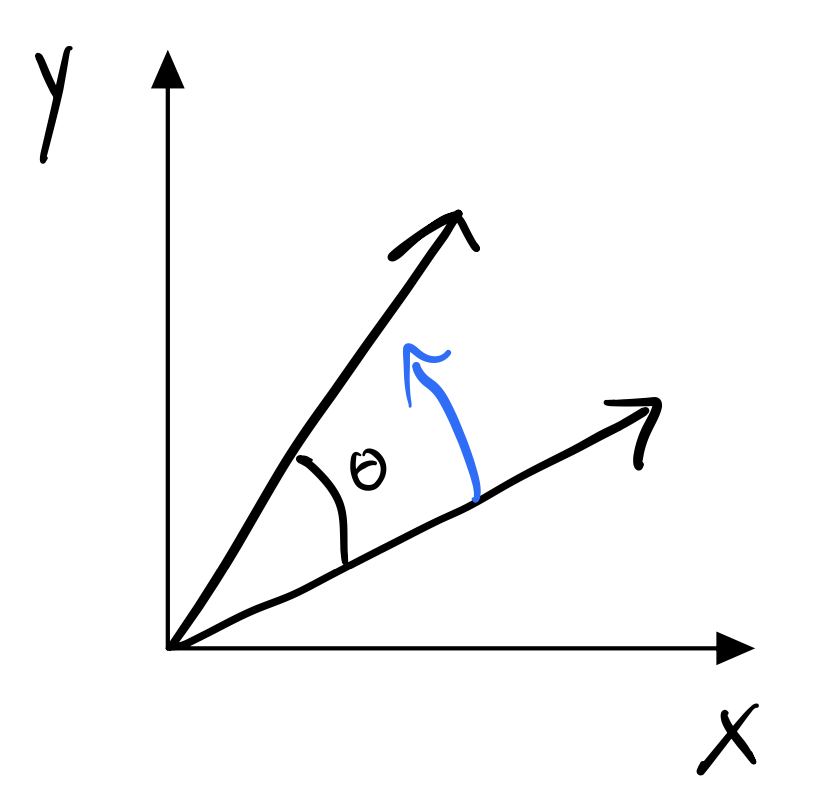
\includegraphics[scale=0.35]{Lectures/Images/lec2-rotation.png}
    \end{center}
    
\end{center}
we have:
\begin{equation}
    R = \m{\cos\theta & -\sin\theta & 0 \\ \sin\theta & \cos\theta & 0 \\ 0 & 0 & 1}
\end{equation}

For a boost in the $x'$ direction with velocity $v$, we have:
\begin{equation}
    \Lambda_{\mu}^{\sp\nu} = \m{\gamma & -\beta \gamma & 0 & 0 \\ -\beta \gamma & \gamma & 0 & 0 \\ 0 & 0 & 1 & 0 \\ 0 & 0 & 0 & 1}
\end{equation}
where the parameters obey (in order for $\Lambda$ to preserve the metric):
\begin{equation}
    \gamma^2(1 - \beta^2) = 1
\end{equation}
$\beta = \frac{v}{c} \in (-1, 1)$ as nothing travels faster than the speed of light. Rearranging for $\gamma$, we have the familiar expression:
\begin{equation}
    \gamma = \frac{1}{\sqrt{1 - \beta^2}}
\end{equation}

We can write:
\begin{equation}
    \beta = \tanh\zeta
\end{equation}
where $\zeta \in (-\infty, \infty)$ is the rapidity. In this parameterization:
\begin{equation}
    \gamma = \frac{1}{\sqrt{1-\beta^2}} = \frac{1}{\sqrt{1 - \tanh^2\zeta}} = \cosh\zeta
\end{equation}
where we have used $\cosh^2\zeta = \sinh^2\zeta + 1$. Note then that $\beta\gamma = \sinh\zeta$. So we can write the boost transformation as:
\begin{equation}
    \Lambda = \m{\cosh\zeta & -\sinh\zeta & 0 & 0 \\ -\sinh\zeta & \cosh\zeta & 0 & 0 \\ 0 & 0 & 1 & 0 \\ 0 & 0 & 0 & 1}
\end{equation}
Which looks quite analogous to what we had with the spatial rotations, except we have replaced the trigonometric functions with their hyperbolic counterparts. Indeed, we can view boosts as hyperbolic rotations.

Under a boost, we have:
\begin{equation}
    \m{x'^0 \\ x'^1} = \m{\gamma & -\beta\gamma \\ -\beta\gamma & \gamma}\m{x^0 \\ x^1} = \m{\gamma x^0 - \beta\gamma x^1 \\ \gamma x^1 - \beta\gamma x^0}
\end{equation}
In the nonrelativistic limit of $v/c \ll 1$:
\begin{equation}
    \gamma = (1-\beta^2)^{-\frac{1}{2}} \approx 1 + \frac{1}{2}\beta^2
\end{equation}
so:
\begin{equation}
    x'0 \approx x^0, \quad x'^1 = x' - \frac{v}{c}\cdot c t
\end{equation}
so we recover the expressions for old (Galilean) boosts. So classical physics was not wrong per se, it just emerges as the nonrelativistic limit of the correction theory. But when we look at relativistic physics (e.g. electromagnetic waves, high-energy particle scattering...) we need to use the relativistic theory.

On Tuesday, we discussed the 10 dimensional Galilean group which quantified the symmetry of classical mechanics. Now, we have modified boosts (i.e. the homogenous part of the Galilean group). The group consisting of 3 spatial rotations + 3 relativistic boosts yields the 6-dimensional Lorentz group, and the 4 spacetime translations yields the 10-dimensional Poincare group.

\subsection{Doppler Effect}
Recall the monochromatic wave solution:
\begin{equation}
    \phi = e^{ik_\mu x^\mu}
\end{equation}
with:
\begin{equation}
    k^2 = k_\mu k^\mu = 0
\end{equation}
\begin{equation}
    \omega = ck^0 = ck, \quad \v{k} = \hat{\v{k}}k = \hat{\v{k}}\frac{2\pi}{\lambda}
\end{equation}
The two heroes of the story are the frequency and $\hat{\v{k}}$ the direction of propagation.

\begin{center}
    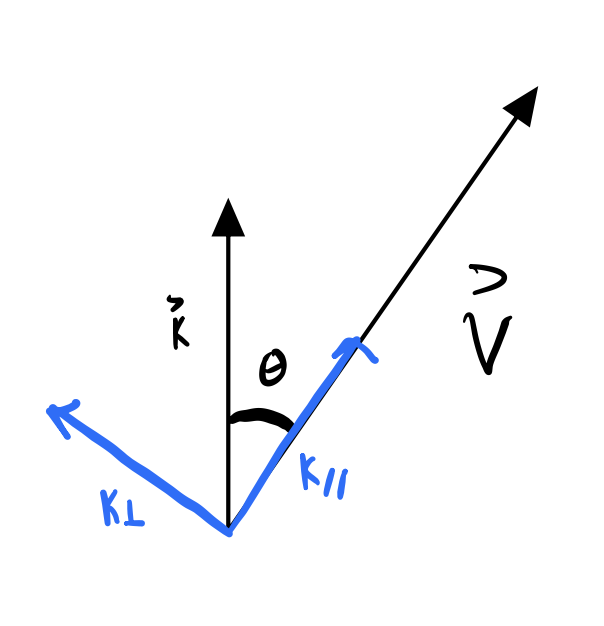
\includegraphics[scale=0.35]{Lectures/Images/lec2-wavevectorboost.png}
\end{center}

The question is now - what does a boosted observer see? We consider the wavevector $\v{k}$ and decompose it into the components perpendicular and parallel to the boost velocity. $\theta$ is the angle between the two vectors. Let us calculate:
\begin{equation}
    k'^\mu = \Lambda^{\mu}_{\sp\nu}k^\nu
\end{equation}
We have:
\begin{equation}
    k'^0 = \gamma(k^0 - \gv{\beta}\cdot\v{k}) = \gamma(k^0 - \beta k_\parallel)
\end{equation}
\begin{equation}
    k'_\parallel = \gamma(k_\parallel - \beta k^0)
\end{equation}
\begin{equation}
    \v{k}'_\perp = \v{k}_\perp
\end{equation}
the last equality follows from the fact that the $\Lambda$ matrix is trivial in this sector.

A good consistency check is that:
\begin{equation}
    k'^2 = k'_\mu k'^\mu = 0
\end{equation}
which you can verify. This tells us that the boosted observer still sees the EM wave propagating at speed:
\begin{equation}
    k'^0 = \abs{\v{k}'}
\end{equation}
This is not something to be surprised about - the formalism was built for this to be true.

If the speed of propagation is not different, what is different? Well, let's look at the $k'^0$ relation. We can write this as:
\begin{equation}
    \omega' = \gamma\omega(1 - \beta\cos\theta)
\end{equation}
So, we see a different frequency, which is the Doppler effect! The direction of propagation is also modified:
\begin{equation}
    \tan\theta = \frac{\abs{\v{k}_\perp}}{k_\parallel}, \quad \tan\theta' = \frac{\abs{\v{k}'_\perp}}{k'_\parallel} =  \frac{\abs{\v{k}_\perp}}{\gamma(k_\parallel - \beta k^0)}
\end{equation}
Since the denominator changes, so too must the angle.

Note the special case of the frequency relation when $\theta = \pi/2$, then:
\begin{equation}
    \omega' = \gamma\omega
\end{equation}
so the shift is manifestly relativistic.

\subsection{Teaser - Relativistic Formulation of Maxwell Theory}
You might say - hey, weren't we studying Maxwell theory the whole time? Indeed we were studying the wave equation, but there is more to Maxwell theory than this! We have to talk about two things:
\begin{itemize}
    \item The dynamics of (charged) particles in electromagnetic fields
    \item The dynamics of the electromagnetic field itself
\end{itemize}

Consider the Lorentz force; suppose we have particle with spatial coordinate $\v{x}(t)$ and charge $q$. In the presence of EM fields, the equation of motion is given by:
\begin{equation}
    \dod{(m\dot{\v{x}})}{t} = \dod{\v{p}}{t} = q(\v{E} + \v{v}\times\v{B})
\end{equation}
These equations are written in a highly inconvenient way for our purposes, as they treat time and space very differently. Time is a label and $\v{x}$ is the position of interest. But for us, we want to package things in terms of 4-vectors/spacetime coordinates $x^\mu = (x^0 = ct, \v{x})$. Thus the above formulation is very inconvenient, e.g., to see how Lorentz transformations work in this theory. We will see how we can formulate the Maxwell theory in a relativistically covariant fashion next time.
\section{Relativistic Formulation of a Free Particle}

At the end of last week, we discovered that the wave equation (in Maxwell theory) must hold in all inertial frames, and as such the notion of boosts in Maxwell theory is different from the Galilean version in classical mechanics. Today what we will do is follow Einstein, and take the attitude that all physical laws must be Lorentz invariance.

To this end, we will need to be generalize the idea of the coordinate $\v{x}(t)$. In classical mechanics, the momentum $\v{p} = m\dot{\v{x}}$ is conserved, and can take on any value. But in the relativistic theory $\abs{\dot{\v{x}}}$ is bounded above by the speed of light. Some kind of reformulation is necessary. We also have the EM fields $\v{E}(\v{x}, t), \v{B}(\v{x}, t)$ - these are already coming out of a Lorentz invariant theory, but we can rewrite the Maxwell equations such that they are manifestly Lorentz covariant.

\begin{center}
    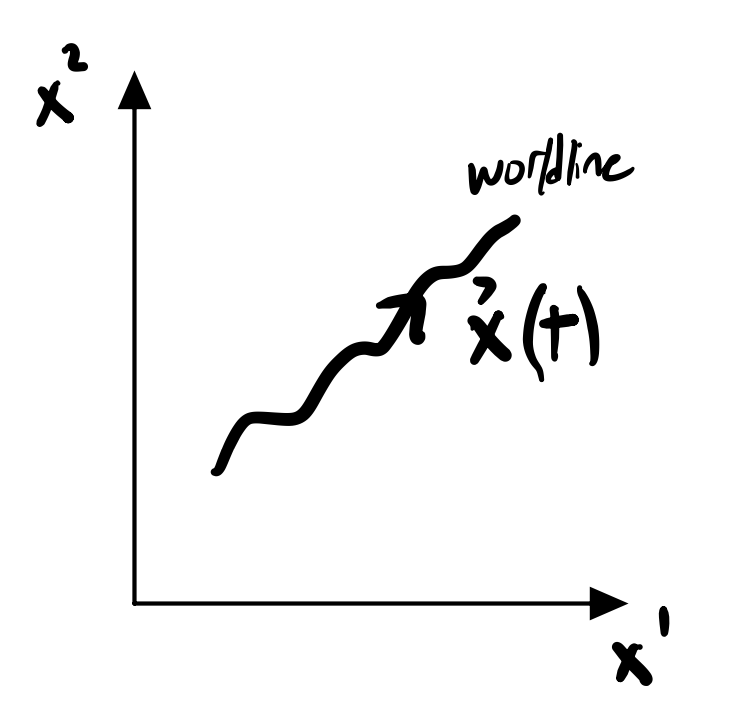
\includegraphics[scale=0.35]{Lectures/Images/lec3-worldline.png}
\end{center}

In classical mechanics, we write down the Lagrangian:
\begin{equation}
    \mathcal{L} = \frac{1}{2}m\dot{\v{x}}^2 - U(\v{x})
\end{equation}
and then solve the EL equations to find the trajectories. 

\subsection{Parametrization}
However, for a relativistically covariant formulation, we would like to put $\v{x}, t$ on the same footing. To this end, we can introduce a parameter $\lambda$, and describe the worldline of the particle as:
\begin{equation}
    x^\mu = x^\mu(\lambda)
\end{equation}
with $\mu = 0, 1, 2, 3$. This might look outlandish, but we do such parametrizations in simpler contexts. For example, consider a line in 2D space:

\begin{center}
    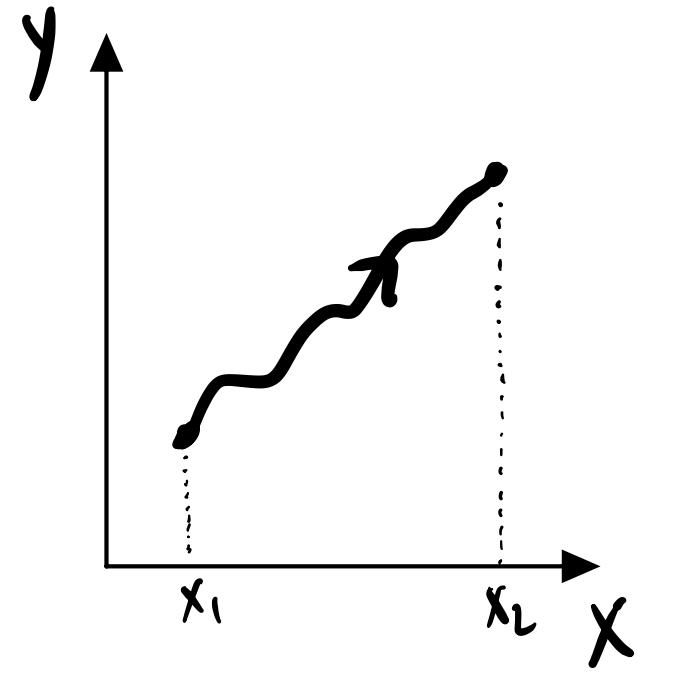
\includegraphics[scale=0.35]{Lectures/Images/lec3-yxpath.png}
\end{center}

Then we could either write $y = y(x)$, or we could write $y = y(\lambda), x = x(\lambda)$ and make them depend on a common parameter:
\begin{equation}
    x = \lambda, y = \lambda^2, \lambda \in [0, 1]
\end{equation}
In doing so, we actually introduced an additional symmetry in the form of reparametrization invariance; indeed we can have $x, y$ in terms of an arbitrary (monotonic, positive) function of $\lambda$:
\begin{equation}
    x= f(\lambda), y = f^2(\lambda), \lambda \in [0, 1]
\end{equation}
This can be useful for calculations in various contexts. For example, suppose we were interested in calculating the length of the line:

\begin{center}
    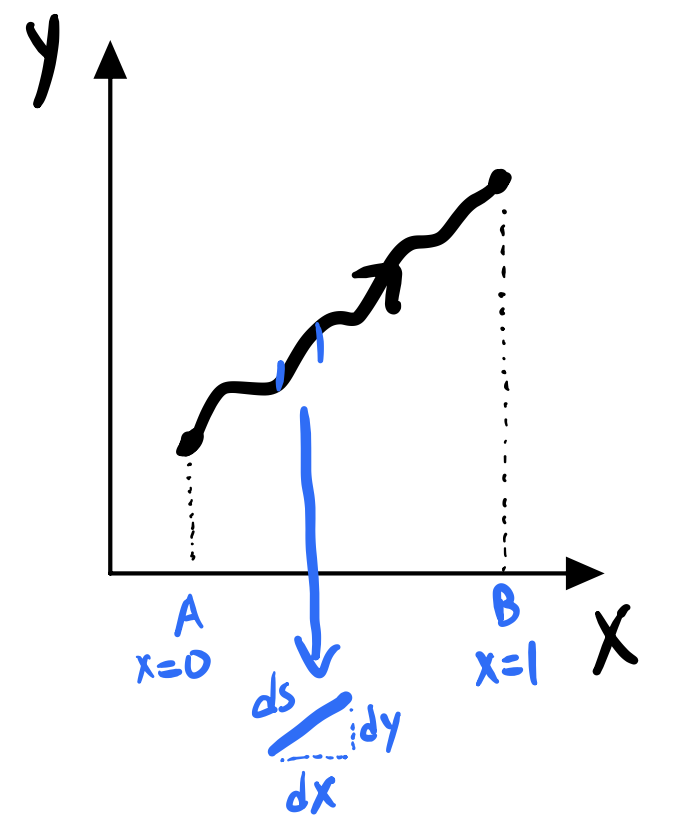
\includegraphics[scale=0.35]{Lectures/Images/lec3-lineelement.png}
\end{center}

Then:
\begin{equation}
    L = \int_A^B ds = \int_A^B \sqrt{dx^2 + dy^2} = \int_0^1 dx \sqrt{1 - \left(\dod[]{y}{x}\right)^2} = \int_0^1 dx\sqrt{1 + y'^2}
\end{equation}

But if $x = x(\lambda), y = y(\lambda)$ for some parameter $\lambda$, we could then write:
\begin{equation}
    ds^2 = (dx(\lambda))^2 + (dy(\lambda))^2 = \left(\dod{x}{\lambda}d\lambda\right)^2  + \left(\dod{y}{\lambda}d\lambda\right)^2 = d\lambda^2\left(\dot{x}^2 + \dot{y}^2\right)
\end{equation}
So:
\begin{equation}
    L = \int_A^B ds = \int_A^B \sqrt{d\lambda^2\left(\dot{x}^2 + \dot{y}^2\right)} = \int_A^B d\lambda\sqrt{\dot{x}^2 + \dot{y}^2}
\end{equation}
the length calculation is now symmetric in $x, y$. If we replace $\lambda \to f(\lambda)$, the length should not change (for it shouldn't matter on the parameterization of the curve!) This must be a symmetry of the integral, and indeed we can easily check that it is. Under $\lambda \to f(\lambda)$:
\begin{equation}
    x^\mu = \frac{dx^\mu}{d\lambda} \to \frac{dx^\mu}{df(\lambda)} = \frac{dx^\mu}{d\lambda}\frac{d\lambda}{df(\lambda)}
\end{equation}
and the same for $y^\mu$. Thus the length becomes:
\begin{equation}
    L = \int_A^B df(\lambda)\sqrt{\left(\frac{dx^\mu}{df(\lambda)}\right)^2 + \left(\frac{dy^\mu}{df(\lambda)}\right)^2} = \int_A^B d\lambda \dot{f} \sqrt{\left(\frac{\dot{x}}{\dot{f}}\right)^2 + \left(\frac{\dot{y}}{\dot{f}}\right)^2} = \int_A^B d\lambda\sqrt{\dot{x}^2 + \dot{y}^2}
\end{equation}
which we can see is invariant (as it should be).

\subsection{Parametrizing Worldlines and Time Dilation}
Back to our problem of parametrizing worldlines. We can repeat the idea from the simple context here, by describing the particle worldine as $x^\mu(\lambda)$. Other than the fact that the time component has a different sign:
\begin{equation}
    ds^2 = -(dx^0)^2 + (dx^1)^2 + (dx^2)^2 + (dx^3)^2
\end{equation}
we can play the same game as before; with $x^\mu = x^\mu(\lambda)$:
\begin{equation}
    ds^2 = d\lambda^2\left(-(\dot{x}^0)^2 + (\dot{x}^1)^2 + (\dot{x}^2)^2 + (\dot{x}^3)^2\right) = d\lambda^2 \dot{x}^\mu \dot{x}_\mu = d\lambda^2 \dot{x}^\mu \dot{x}^\nu \eta_{\mu\nu}
\end{equation}
This line element is reparametrization invariant, but also is Lorentz invariant (as it is written as a contraction with the Minkowski metric).

To do physics, we want to fix reparametrization symmetry. It is natural to fix $x^0(\lambda) = \lambda c$, so then $t(\lambda) = \lambda$. The logic is we have four functions, and we can freely reparametrize - using this symmetry, we may pick the time function to be simple. Let's see what happens to $ds^2$ when we do this:
\begin{equation}
    ds^2 = dt^2\left(-c^2 + \left(\dod{\v{x}}{t}\right)^2\right) = -c^2dt^2\left(1 - \gv{\beta}^2\right)
\end{equation}
with $\gv{\beta} = \frac{\v{v}}{c} = \frac{\dot{\v{x}}}{c}$. A natural definition is:
\begin{equation}
    d\tau^2 = dt^2(1 - \gv{\beta}^2)
\end{equation}
so:
\begin{equation}
    ds^2 = -c^2d\tau^2
\end{equation}
$\tau$ is called the proper time. In the frame where $\gv{\beta} = 0$, we can see from the above $\tau = t$; it thus has the interpretation as the time in the inertial frame in which the particle is at rest momentarily. The relation between $t, \tau$ can be written as:
\begin{equation}
    dt = \gamma d\tau
\end{equation}
with:
\begin{equation}
    \gamma^2 = \frac{1}{1 - \gv{\beta}^2}
\end{equation}
This is the celebrated time dilation formula. This says that things that take time $d\tau$ in the frame of the particle are dilated/increased by $\frac{1}{1-\gv{\beta}^2}$ in the frame of the external observer. As a concrete example, if a particle has a lifetime $T$, someone who sees the particle moving will see its lifetime as $\gamma T$. You may be familiar with the fact that cosmic rays create muons with, $T = 2.2 \cdot 10^{-6}\si{s}$. In the muon frame, it can only travel $2. 2 \cdot 10^{-6}\si{s} \cdot 3 \times 10^{8}\si{ms^{-1}} = 0.66\si{km}$. But we observe that cosmic ray muons propagate for hundreds of kilometers, and the explanation is that their lifetime is extended via time dilation.

\subsection{Lagrangian for Relativistic Particle}
The usual Lagrangian:
\begin{equation}
    \mathcal{L} = \frac{1}{2}m\dot{\v{x}}^2 - U(\v{x})
\end{equation}
does not work in our relativistic formulation as the particle could have any velocity, and velocities are bounded by the speed of light. Further, the action $S = \int dt \mathcal{L}$ is not invariant under Lorentz transformations. Can we modify this Lagrangian in some way? A very natural candidate is:
\begin{equation}\label{eq:LIaction}
    S = A\int d\lambda \sqrt{-\dot{x}_\mu \dot{x}^\mu}.
\end{equation}
This is automatically Lorentz invariant. It is also reparametrization invariant, so let us fix the reparametrization symmetry by taking $\lambda = t$:
\begin{equation}
    S = \tilde{A}\int dt \sqrt{1 - \frac{\dot{\v{x}^2}}{c^2}}.
\end{equation}
This is now invariant under the boosts that we defined last week - even though it looks like it mixes $x/t$ because they are written separately, we know from the form of Eq. \eqref{eq:LIaction} that it is indeed invariant. It is also now clear why we took the minus sign there; we want the argument of the square root to be always positive.

We are not quite done yet. We have to check that the action passes basic scrutiny. One sanity check is that in the non-relativistic limit of $\dot{\v{x}} \ll c$. Using the binomial approximation:
\begin{equation}
    S = \tilde{A}\int dt\left[1 - \frac{1}{2}\frac{\dot{\v{x}}^2}{c^2} + O(\frac{\abs{\dot{\v{x}}}^4}{c^4})\right]
\end{equation}
This motivates the choice that $\tilde{A} = -mc^2$:
\begin{equation}
    S = \int dt\left(-mc^2 + \frac{1}{2}m\dot{\v{x}}^2 + \ldots \right)
\end{equation}
This looks very good! We have the kinetic term with the correct normalization, and the first term can be thought of the rest energy of the particle $U = mc^2$. Note that the zero of the energy has been fixed - in regular classical mechanics, we usually have a freedom to choose what our ``zero'' is, but it does matter here.

The bottom line is our action:
\begin{equation}
    S = -mc^2\int dt\sqrt{1 - \frac{\dot{\v{x}}^2}{c^2}}
\end{equation}
has the properties that it is Lorentz invariant and it produces the correct formula in the low-velocity limit. This is the action we will be working with!

\subsection{Relavistic energy and momentum}

We want to turn the crank of the classical mechanics machinery and write down the Euler-Lagrange equations, and define energy and momentum. The E-L equations are:
\begin{equation}
    \dod{}{t}\ddpd{\LL}{\dot{x}^i} = \ddpd{\LL}{x^i}
\end{equation}
for $i = 0$. Since the Lagrangian is independent of $x^i$:
\begin{equation}
    \dod{}{t}\ddpd{\LL}{\dot{x}^i} = 0
\end{equation}
Thus we can define the (conserved) momentum:
\begin{equation}
    p^i = \frac{m\dot{x}^i}{\sqrt{1-\frac{\v{v}^2}{c^2}}} = \gamma m\dot{x}^i
\end{equation}
So the difference between the non-relativistic case ($m\dot{x}^i$) and relativistic case ($\gamma m\dot{x}^i$) is that $\gamma m$ is an effective ``relativistic mass''; the faster the particle travels, the heavier it becomes/harder it becomes to change its momentum (and hence it can never surpass the speed of light).

We can also write down the Hamiltonian (equal to the energy because $\LL$ does not depend on time):
\begin{equation}
    H = E = p_i \dot{x}^i - \LL = \gamma mc^2
\end{equation}
where again the energy becomes larger and larger the more the particle approaches the speed of light.

You can easily convince yourself that:
\begin{equation}\label{eq:Eprelation}
    E^2 = c^2\abs{\v{p}}^2 + (mc^2)^2
\end{equation}
This is an interesting formula for the following reason. $(E, \v{p})$ are a scalar and vector under rotations. Because rotations are a subgroup of Lorentz transformations, they presumably can be combined to a four-vector $p^\mu = (\frac{E}{c}, \v{p})$. $p^\mu \to p'^\mu = \Lambda^{\mu}_{\sp\nu}p^\nu$ under Lorentz transformations. In this language, Eq. \eqref{eq:Eprelation} has the nice inrepretation:
\begin{equation}
    p_\mu p^\mu = -(mc)^2
\end{equation}
So the combination $p_\mu p^\mu$ is a Lorentz invariant quantity.

Next time, we will look at the relativistic formulation of Maxwell's theory; we have fields $\v{E}(\v{x}, t), \v{B}(\v{x}, t)$, which satisfy:
\begin{equation}
    \nabla \cdot \v{E} = \frac{\rho}{\e_0}
\end{equation}
\begin{equation}
    \nabla \cdot \v{B} = 0
\end{equation}
\begin{equation}
    \nabla \times \v{B} - \frac{1}{c}\v{E} = \mu_0 \v{J}
\end{equation}
\begin{equation}
    \nabla \times \v{E} + \dot{\v{B}} = 0
\end{equation}
we will repackage these in such a way that it is clearer to see that they are Lorentz invariant. We will then combine our work on a relativistically invariant formulation of the mechanics of a particle with this.
\section{Relativistic Formulation of Maxwell Theory}

A small comment from last class - we discussed the fact that we could package the energy and momentum into a four vector:
\begin{equation}
    (E, \v{p}) = p^\mu
\end{equation}
and that:
\begin{equation}
    p_\mu p^\mu = p^\mu p^\nu \eta_{\mu\nu} = -(mc)^2
\end{equation}
is a Caismir of the Poincare group/is a Poincare invariant. That is to say - the above is an invariant under boosts/rotations/translations, and has the interpretation that it is the mass of the particle, which is unchanged under all such transformations.

Today, we move onto the relativistic formulation of the Maxwell theory - in your EM courses you have surely seen the 4 Maxwell equations:
\begin{equation}
    \nabla \cdot \v{E} = \frac{\rho}{\e_0}
\end{equation}
\begin{equation}
    \nabla \cdot \v{B} = 0
\end{equation}
\begin{equation}
    \nabla \times \v{B} - \frac{1}{c}\v{E} = \mu_0 \v{J}
\end{equation}
\begin{equation}
    \nabla \times \v{E} + \dot{\v{B}} = 0
\end{equation}
We suspect ahead of time that these are Lorentz invariant (as the wave equation is a consequence of these equations, and it is Lorentz invariant) but there is a way we can write them down such that they are manifestly so.

\subsection{Maxwell under Rotations}
Let's start with rotations, which are a subset of Lorentz transformations. It is not hard to show that the Maxwell equations as written above are already invariant under rotations - let's work this out. The charge density is a scalar, and so:
\begin{equation}
    \rho'(\v{x}') = \rho(\v{x})
\end{equation}
Where $\v{x}' = R\v{x}$, or in index notation, $x^i = R^{ij}x^j$. What of the vector quantities? $\v{E}, \v{B}, \v{J}$ are vector fields, which have a direction at each point in space:

\begin{center}
    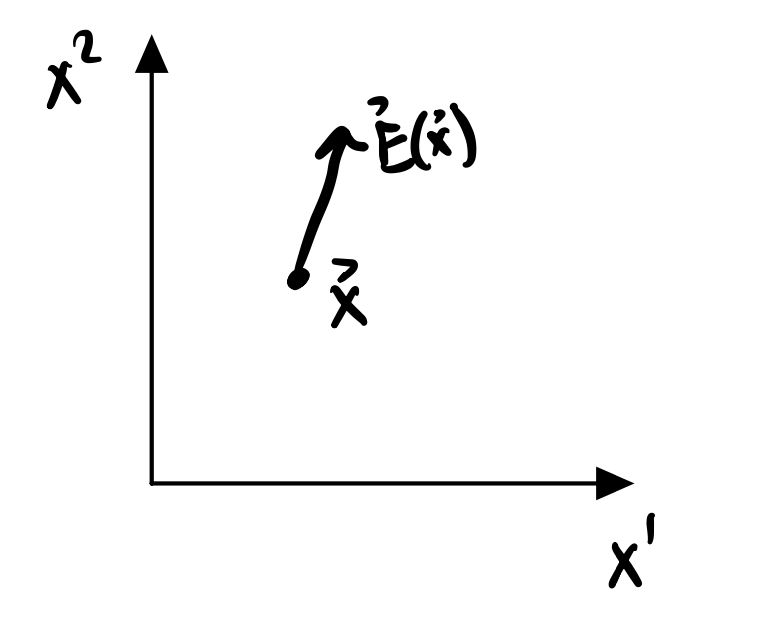
\includegraphics[scale=0.35]{Lectures/Images/lec4-vectorfield.png}
\end{center}

and you can convince yourself that vector fields have the following transformation:
\begin{equation}
    E'_i(\v{x}')dx'^i = E_i(\v{x})dx^i
\end{equation}

\subsection{Gauge Fields}

What we would like to do is generalize this to all Lorentz transformations, where four-vectors $x^\mu = (t, \v{x})$ transform as:
\begin{equation}\label{eq:spacetimecoordLorentztransformation}
    x'^\mu = \Lambda^{\mu}_{\sp\nu}x^\nu.
\end{equation}
The issue now becomes that it is unclear how $\v{E}, \v{B}$ (which are \emph{not} 4-vectors) transform. The main hint is that we may write the electric and magnetic fields in terms of a scalar and vector potential:
\begin{equation}
    \v{E} = -\nabla \phi - \dot{\v{A}}
\end{equation}
\begin{equation}
    \v{B} = \nabla \times\v{A}
\end{equation}
there is a sense in which $\phi, \v{A}$ are more fundamental than $\v{E}, \v{B}$, which we will see later in the lecture.Now, we are back to a problem that we have previously encountered. We have a scalar $\phi$ and a vector $\v{A}$, so it makes sense to package them into a single four-vector, known as the gauge field:
\begin{equation}
    A^\mu = (\frac{\phi}{c}, \v{A})
\end{equation}
The question then becomes whether or not this is a useful definition, and the answer is yes! 

Under Lorentz transformations, we expect:
\begin{equation}
    A_\mu(x')dx'^\mu = A_\nu(x)dx^\nu
\end{equation}
before we move on, it's worth picking apart exactly what this means; if we divide both sides by $dx^\nu$:
\begin{equation}
    A_\mu'(x')\frac{dx'^\mu}{dx^\nu} = A_\nu(x)
\end{equation}

Now, the derivative we can read off from Eq. \eqref{eq:spacetimecoordLorentztransformation}:
\begin{equation}
    \frac{dx'^\mu}{dx^\nu} = \Lambda^{\mu}_{\sp\nu}
\end{equation}
so then:
\begin{equation}
    A_\mu'(x')\Lambda^{\mu}_{\sp\nu}= A_\nu(x)
\end{equation}

\subsection{Field Strength}
Now, we have to check what the implication this is for on the $\v{E}, \v{B}$ - the answer is that we can define the field strength of the gauge field:
\begin{equation}
    F_{\mu\nu} = \p_\mu A_\nu - \p_\nu A_\mu
\end{equation}
where $\p_\mu = \ddpd{}{x^\mu}$. I have a suspicion that $F_{\mu\nu}$ has something to do with $\v{E}, \v{B}$. The first reason is that $F_{\mu\nu}$ is a $4\times 4$ antisymmetric matrix:
\begin{equation}
    F_{\mu\nu} = -F_{\nu\mu}
\end{equation}
which contains 6 independent components, which matches the total number of independent components stored in the $\v{E}, \v{B}$. The other reason is that $F_{\mu\nu}$ is gauge invariant. Last quarter, you noticed that, for an arbitrary scalar function $\chi$, we could transform the scalar/vector potential as:
\begin{equation}
    \phi' = \phi - \p_t \chi, \quad \v{A}' = \v{A} + \nabla \chi
\end{equation}
and under such a transformation $\v{E}, \v{B}$ are invariant. Such transformations are known as gauge transformations, and are labelled by an arbitrary scalar function of spacetime. In order to discuss what happens to $F_{\mu\nu}$ under such transformations, we first act how the gauge field $A_\mu(x)$ transforms under such a transformation:
\begin{equation}
    A_\mu'(x) = A_\mu(x) + \p_\mu \chi
\end{equation}
Let's check this for the 0-th/time component:
\begin{equation}
    A_0' = A_0 + \ddpd{}{x^0}\chi \implies -\frac{\phi'}{c} = -\frac{\phi}{c} + \dpd{}{(ct)}\chi \implies \phi' = \phi - \p_t \chi
\end{equation}
and the story for the spatial components is analogous. With this, let's check how the field strength transforms:
\begin{equation}
    F_{\mu\nu}' = \p_\mu A_\nu' - \p_\nu A_\mu' = \p_\mu(A_\nu + \p_\nu\chi) - \p_\nu(A_\mu + \p_\mu \chi) = F_{\mu\nu} + \p_\mu\p_\nu\chi - \p_\nu\p_\mu\chi = F_{\mu\nu}
\end{equation}
it is invariant! So now we're pretty confident that the components of $F$ will give the components of the $\v{E}/\v{B}$ fields. Let's work them out:
\begin{equation}
    F_{i0} = -F_{0i} = \p_i A_0 - \p_0 A_i = -\frac{1}{c}\p_i \phi - \p_0 A_i = \frac{1}{c}E_i
\end{equation}
\begin{equation}
    F_{12} = -F_{21} = \p_1 A_2 - \p_2 A_1 = \e_{3jk}\p_j A_k = B_3
\end{equation}
(where in the last equality we recall that $B_i = \e_{ijk}\p_j A_k$). Thus for the general component of the B-field:
\begin{equation}
    B_i = \frac{1}{2}\e_{ijk}F_{jk}
\end{equation}
the $\frac{1}{2}$ coming from the fact that when we do the $j, k$ summations we get two nonzero terms. The bottom line of this discussion:
\begin{equation}
    F_{\mu\nu} = \m{0 & -\frac{1}{c}E_1 & -\frac{1}{c}E_2 & -\frac{1}{c}E_3 \\ \frac{1}{c}E_1 & 0 & B_3 & -B_2 \\ \frac{1}{c}E_2 & - B_3& 0 & B_1 \\ \frac{1}{c}E_3 & B_2 & -B_1 & 0}
\end{equation}
why did we do all of this? When we first wrote down the Maxwell equations, we had confusion about how $\v{E}, \v{B}$ transform under Lorentz transformations. Now we have answered it - we can combine $\v{E}, \v{B}$ into $F_{\mu\nu}$ and it is easy to see how this transforms, because we know how $A_\mu$ transforms under Lorentz:
\begin{equation}
    F'^{\mu\nu}(x') = \Lambda^{\mu}_{\sp\lambda}\Lambda^{\nu}_{\sp\rho}F^{\lambda\rho}(x)
\end{equation}
This looks very abstract, but it answers very physical questions. Suppose we have a charged particle, eminating an $\v{E}$-field. I could then get on a bike\footnote{Assuming I was very good at riding a bike and I could go close to the speed of light...} and ask what $\v{E}, \v{B}$-fields I observe - this allows us to answer it.

So far, we have just written down a bunch of definitions we hope would be useful. We had Maxwell's equations, and we wanted to make sure they were invariant under Lorentz transformations. Now, we are in a position to go back to this question, and ask if we can write Maxwell's equations in a way where the Lorentz invariance is manifest.

\subsection{Lorentz Covariant Maxwell Equations}
We require one more definition, that of the dual field strength. We have the field strength:
\begin{equation}
    F_{\mu\nu} = \p_\mu A_\nu - \p_\nu A_\mu
\end{equation}
and then its dual is defined by:
\begin{equation}
    {F^*}^{\alpha\beta} = \tilde{F}^{\alpha\beta} \coloneqq \frac{1}{2}\e^{\alpha\beta\gamma\delta}F_{\gamma\delta}
\end{equation}
where:
\begin{equation}
    \e^{0123} = 1
\end{equation}
and every time two indices are flipped we get a $-1$ sign. The $\frac{1}{2}$ in the definition is there to account for the fact that we get two factors in the summation over $\gamma, \delta$. 

We can explicitly work out the components:
\begin{equation}
    \tilde{F}_{\mu\nu} = \m{0 & B_1 & B_2 & B_3 \\ -B_1 & 0 & \frac{1}{c}E_3 & -\frac{1}{c}E_2 \\ -B_2 & -\frac{1}{c}E_3 & 0 & \frac{1}{c}E_1 \\ -B_3 & \frac{1}{c}E_2 & -\frac{1}{c}E_1 & 0}
\end{equation}
from which we can see that $F, \tilde{F}$ are related via $\v{E} \to c\v{B}, c\v{B} \to -\v{E}$. This is the beginning of a rabbit hole known as electromagnetic duality, and it has lead theorists to believe that there exist magnetic monopoles.

We claim that the dual tensor satisfies:
\begin{equation}
    \p_\mu \tilde{F}^{\mu\nu} = 0
\end{equation}
Let's prove this; fully writing out the dual tensor:
\begin{equation}
    \tilde{F}^{\mu\nu} = \e^{\mu\nu\gamma\delta}(\p_\gamma A_\delta - \p_\delta A_\gamma)
\end{equation}
Now taking the derivative;
\begin{equation}
    \p_\mu \tilde{F}^{\mu\nu} = \e^{\mu\nu\gamma\delta}(\p_\mu\p_\gamma A_\delta - \p_\mu \p_\delta A_\gamma)
\end{equation}
Note that the derivative terms are symmetric under $\mu \leftrightarrow \gamma$ and $\mu \leftrightarrow \delta$, but $\e^{\mu\nu\gamma\delta}$ is antisymmetric under such interchanges; hence the derivative vanishes:
\begin{equation}
    \boxed{\p_\mu \tilde{F}^{\mu\nu} = 0}
\end{equation}
and we call this the \emph{Bianchi identity}. Actually, it is four equations, one for each $\nu = 0, 1, 2, 3$. We can write this identity in terms of electric and magnetic fields:
\begin{equation}
    \nabla \cdot \v{B} = 0
\end{equation}
\begin{equation}
    \nabla \times \v{E} + \dot{\v{B}} = 0
\end{equation}
which we can see are just two of the Maxwell equations - the equations are really Lorentz covariant, because we can write them in terms of $\tilde{F}^{\mu\nu}$, so if they are satisfied in one frame we can easily deduce that they are in a boosted frame.

We then have the other two equations which don't straightforwardsly follow from the Bianchi identity:
\begin{equation}
    \nabla \cdot \v{E} = \frac{\rho}{\e_0}
\end{equation}
\begin{equation}
    \nabla \times \v{B} - \frac{1}{c}\dot{\v{E}} = \mu_0\v{J}
\end{equation}

The charge and current densities satisfy the continuity equation:
\begin{equation}
    \dot{\rho} + \nabla \cdot \v{J} = 0
\end{equation}
at this point, we're Pavlovian dogs who start drooling whenever we see a scalar and a vector together, so we're motivated to define:
\begin{equation}
    J^\mu = (c\rho, \v{J})
\end{equation}
wherein the continuity equation just reads:
\begin{equation}
    \p_\mu J^\mu = 0 
\end{equation}

Under Lorentz transformations:
\begin{equation}
    J'^\mu(x')dx'_\mu = J^\nu(x)dx_\nu
\end{equation}

So let's get back to the remaining two Maxwell equations; you can convince yourself that:
\begin{equation}
    \boxed{\p_\mu F^{\mu\nu} = -\mu_0 J^\nu}
\end{equation}
which is the relativistically covariant form of the Maxwell equations relating the fields to charges/currents.

One thing to point out - when we write this, one thing that is obvious is that if we can write this at all, the current must be conserved. The reason is that if that if I take the derivative $\p_\nu$:
\begin{equation}
    \p_\nu \p_\mu F^{\mu\nu} = -\mu_0 \p_\nu J^\nu
\end{equation}
on the LHS we have a trivial zero (symmetric derivative of an antisymmetric tensor) so:
\begin{equation}
    \p_\nu J^\nu = 0
\end{equation}
the current must be conserved. Said another way, the electromagnetic field can only couple consistently to conserved currents.

A comment - on Tuesday, we discussed the dynamics of free particles. We might ask whether we've solved the problem of charged particles here - the answer is not quite, since throughout we've assumed $\rho, \v{J}$ are smooth and a charged pointlike particle would give rise to a delta-function concentrated charge/current. But we'll see how to deal with this later.

\subsection{Lagrangian Formulation}
We have found the Maxwell equations:
\begin{equation}
    \p_\mu \tilde{F}^{\mu\nu} = 0
\end{equation}
\begin{equation}
    \p_\mu F^{\mu\nu} = -\mu_0 J^\nu
\end{equation}
and we want to know whether we can get these equations from Euler-Lagrange equations that follow from some Lagrangian.

First, we review the situation in point-particle mechanics. Then, we generalize to field theory. Finally, we will specialize to E\& M.

In classical mechanics, we have generalized coordinates $q_i(t)$ for $i = 1, \ldots n$. The action is then:
\begin{equation}
    S = \int dt \mathcal{L}(q_i, \dot{q}_i)
\end{equation}
for $\mathcal{L} = T - U$. The Euler-Lagrange equations are then:
\begin{equation}
    \dod{}{t}\dpd{\LL}{\dot{q}_i} = \dpd{\LL}{q_i}
\end{equation}
and you have solved this, e.g., when $T = \frac{1}{2}\sum_i m_i \dot{q}_i^2$ and $U = U(q_1, \ldots q_n)$. 

We now want to promote these coordinates to fields, $q_i(t) \to \phi_i(t, \v{x})$, and we shall continue with this next lecture.
\section{Lagrangian for EM field}

In relativistic notation, Maxwell's equations are:

\begin{equation}
    \p_\mu \tilde{F}^{\mu\nu} = 0
\end{equation}
\begin{equation}
    \p_\mu F^{\mu\nu} = -\mu_0 J^{\nu}
\end{equation}
where:
\begin{equation}
    F_{\mu\nu} = \p_\mu A_\nu - \p_\nu A_\mu
\end{equation}
\begin{equation}
    \tilde{F}^{\mu\nu} = \frac{1}{2}\e^{\mu\nu\rho\sigma}F_{\rho\sigma}
\end{equation}
we then raised the question: could we derive these equations from a Lagrangian?

\subsection{From particles to fields}
Brief review of classical mechanics of particles - we consider an action:
\begin{equation}
    S = \int dt \mathcal{L}(q_i(t), \dot{q}_i(t))
\end{equation}
Which, extremizing, we obtain the Euler-Lagrange equations:
\begin{equation}
    \dod{}{t}\dpd{\LL}{\dot{q}_i} = \dpd{\LL}{q_i}
\end{equation}
which are equivalent to Newton's second law.

We now generalize, in two steps. First, we generalize the generalized coordinates $q_i(t)$ to a field $\phi$:
\begin{equation}
    q_i(t) \to \phi(x) = \phi(\v{x}, t)
\end{equation}
Comparing to what we had in the case of particle mechanics, instead of the $i$ index we have the position $\v{x}$ - we have a continuous number of degrees of freedom. Field theory is nothing more than classical mechanics of an infinite degrees of freedom.

We can further generalize:
\begin{equation}
    \phi(x) \to \phi_i(x)
\end{equation}
where $i = 1, \ldots n$. This is not to be confused with the index $i$ for the particle label. This is just saying we have $i = 1, \ldots n$ different fields.

In our application, we take $\phi_i \to A_\mu$. The spacetime index $\mu$ plays the role of $i$. $A_\mu$ is a vector field, and in full gory detail:
\begin{equation}
    A_\mu = A_\mu(x^0, x^1, x^2, x^3)
\end{equation}
with $\mu = 0, 1, 2, 3$. Lorentz transformations act on both indices.

Comment: this is similar to the role of spin in quantum mechanics; we had wavefunctions $\phi(\v{x}, t)$ which we obtained by solving the Schrodinger equation. When we solved for the energy levels of the hydrogen atom, we likely ignored the fact that the electron had spin. But in the presence of the magnetic field, there is a term in the Hamiltonian that acts on the spin, so we add an extra index $\alpha$ to $\psi_{\alpha}(\v{x}, t)$ where $\alpha = \uparrow, \downarrow$. $\mu$ plays an analogous role - we have spin-1.

Going back to the action, we can write (restricting to just one field for now):
\begin{equation}
    S = \int d^4x \mathcal{L}(\phi(x), \p_\mu \phi(x)).
\end{equation}
We want to understand what is the analog of the Euler-Lagrange equations? We will follow the same logic in the particle case - we vary the field $\phi$:
\begin{equation}
    \phi(x) \to \phi(x) + \delta\phi
\end{equation}
where the variation $\delta\phi$ is arbitrary and small\footnote{The proof of the fact that Kusatov has free will is that he can choose any variation he likes, here.}. We then ask by how much does $S(\phi)$ change under the variation, to first order in $\delta \phi$:
\begin{equation}
    \begin{split}
        \delta S &= S(\phi + \delta \phi) - S(\phi) 
        \\ &= \int d^4x\left[\LL(\phi + \delta \phi, \p_\mu \phi + \p_\mu \delta \phi) - \LL(\phi, \p_\mu \phi)\right]
        \\ &= \int d^4x\left[\delta \phi \dpd{\LL}{\phi} + \p_\mu \delta\phi\dpd{\LL}{(\p_\mu \phi)}\right]
        \\ &= \int d^4x\left[\delta \phi \dpd{\LL}{\phi} + \p_\mu\left(\delta \phi \dpd{\LL}{(\p_\mu \phi)}\right) - \delta \phi \p_\mu \dpd{\LL}{(\p_\mu \phi)}\right]
    \end{split}
\end{equation}
Now, the middle term is an integral of a total derivative. We can thus write it as (for $\mu = 0$):
\begin{equation}
    \int d^4x \p_0\left[\left(\dpd{\LL}{(\p_0 \phi)}\right)\delta \phi\right] = \left.\int d^3 x \dpd{\LL}{(\p_0 \phi)}\delta\phi \right|_{x^0 = -\infty}^{x^0 = \infty}
\end{equation}
and we can choose the variation $\delta\phi$ to go to zero at the boundary of time. This is analogously true for the spatial $\mu$s. Thus the total derivative term drops out, and the variation in the action becomes:
\begin{equation}
    \delta S = \int d^4 x \delta \phi(x) \left[\dpd{\LL}{\phi} - \p_\mu \dpd{\LL}{(\p_\mu\phi)}\right] = 0
\end{equation}
and if we want this to hold for all variations $\delta \phi(x)$, we thus obtain:
\begin{equation}
    \dpd{\LL}{\phi} = \p_\mu\dpd{\LL}{(\p_\mu \phi)}
\end{equation}
or in the case of multiple fields:
\begin{equation}
    \boxed{\dpd{\LL}{\phi_i} = \p_\mu\dpd{\LL}{(\p_\mu \phi_i)}}
\end{equation}

\subsection{EM field Lagrangian - no sources}
We want:
\begin{equation}
    S = \int d^4x\mathcal{L}(A_\mu(x), \p_\nu A_\mu(x))
\end{equation}
note that the Lagrangian depends on the gauge potential $A_\mu$ as opposed to the electric/magnetic field. We want to get the Maxwell equations out of the Euler-Lagrange equations:
\begin{equation}
    \dpd{\LL}{A_\nu} = \p_\mu \dpd{\LL}{(\p_\mu A_\nu)}
\end{equation}
What $\LL$ should we choose? First, we have the equation/Bianchi identity:
\begin{equation}
    \p_\mu \tilde{F}^{\mu\nu} = 0
\end{equation}
but this equation is a triviality. This is just true by the definition of the (dual) field strength. So we don't want this from the Lagrangian. What we actually want to derive from the Lagrangian is:
\begin{equation}
    \p_\mu F^{\mu\nu} = -\mu_0 J^\nu
\end{equation}
For simplicity, let's start in the case with $J^\nu = 0$. We then want to reproduce:
\begin{equation}
    \p_\mu F^{\mu\nu} = \p_\mu(\p^\nu A^\nu - \p^\nu A^\mu) = 0.
\end{equation}
$\LL$ should satisfy some properties:
\begin{itemize}
    \item  $\LL$ should be Lorentz invariant - this is because $S$ should be Lorentz invariant, and $d^4x$ is Lorentz invariant.
    \item $\LL$ should be gauge invariant - the Maxwell equation and physics we get out of it should be gauge invariant.
    \item The Euler-Lagrange equation is linear in $A_\mu$ - thus $\LL$ should be quadratic in $A_\mu$.
\end{itemize}

Given these conditions, we have only three objects we could conceivably write\footnote{If you can think of another, please tell Kusatov, and he will immediately run to write a paper on it without you.}:
\begin{itemize}
    \item $-F_{\mu\nu}F^{\mu\nu}$
    \item $-F_{\mu\nu}\tilde{F}^{\mu\nu}$
    \item $-\tilde{F}_{\mu\nu}\tilde{F}^{\mu\nu}$
\end{itemize}
Note that $-\tilde{F}_{\mu\nu}\tilde{F}^{\mu\nu}$ is proportional to $-F_{\mu\nu}F^{\mu\nu}$ and so is not a unique possibility, and $-F_{\mu\nu}\tilde{F}^{\mu\nu}$ is a total derivative and so does not contribute to the physics. We thus have one possibility remaining:
\begin{equation}
    \LL_{\text{EM}} = -\frac{1}{4\mu_0}F_{\mu\nu}F^{\mu\nu}
\end{equation}
The proportionality constant we put there for later convenience, but this is not important for the purposes of the Euler-Lagrange equation. In the next problem set, you can verify that the E-L equation yields precisely $\p_{\mu}F^{\mu\nu} = 0$. This must work - if it did not, there would be no Lagrangian that could possibly works, and we just wasted 2 weeks of your time. Writing $\LL$ in terms of the electromagnetic fields, we have:
\begin{equation}
    \LL_{\text{EM}} = \frac{1}{2\mu_0}\left(\frac{1}{2}\abs{\v{E}}^2 - \abs{\v{B}}^2\right)
\end{equation}
wherein we can immediately see that the Euler-Lagrange procedure would be doomed to fail if we had used $\v{E}, \v{B}$ as the fundamental degrees of freedom.

\subsection{EM field Lagrangian - with sources}
If we want to reproduce the case with sources:
\begin{equation}
    \p_{\mu}F^{\mu\nu} = -\mu_0 J^\nu
\end{equation}
we can simply add the term:
\begin{equation}
    \LL = -\frac{1}{4\mu_0}F^{\mu\nu}F_{\mu\nu} + A_\mu J^\mu.
\end{equation}

But actually there is a problem here. This Lagrangian is \emph{not} gauge invariant. If we perform the gauge transformation:
\begin{equation}
    A_\mu \to A_\mu - \p_\mu \chi
\end{equation}
Then the Lagrangian picks up a new term:
\begin{equation}
    \delta \LL = -J^\mu \p_\mu \chi
\end{equation}

Is this a problem? Actually, no. What we \emph{really} want is not that $\LL$ is gauge invariant, but that the action $S$ is gauge invariant. In other words, does $\delta S$ from making the gauge transformation vanish?
\begin{equation}
    \delta S = \int d^4x \delta \LL = -\int d^4x J^\mu \p_\mu \chi = -\int d^4x \p_\mu[J^\mu \chi]
\end{equation}
In the last line, we wrote things as a total derivative; this is valid as:
\begin{equation}
    \p_\mu [J^\mu \chi] = (\p_\mu J^\mu)\chi + J^\mu (\p_\mu \chi) = J^\mu (\p_\mu \chi)
\end{equation}
as $\p_\mu J^\mu = 0$ (continuity equation/current conservation). Going back to $\delta S$, we can have some discussion about the integral of the total derivative. As we discussed earlier in lecture, this only receives contributions from the boundaries of spacetime. So, the action is invariant under gauge transformations that go to zero rapidly to zero at the boundaries of spacetime. But if we include $\chi$s that do \emph{not} go to zero, we get physically important boundary terms - they are relevant to charge conservation. But in this course we do not consider such cases.

Another point to make - the discussion heavily relies on the fact that the current $J^\mu$ is conserved. If we want the action to be invariant under gauge transformations, we can only couple the electromagnetic field to conserved currents.

\subsection{The stress-energy tensor}
Now, we can ask what this Lagrangian is good for - of course, we already have the Euler-Lagrange equation; another answer is we can get the stress-energy tensor for the EM field. Why is this physically important? You are already viscerally aware of the fact that particles have energy and momenta. But you also expect that the electromagnetic field also has this property. What is the analogue of the energy/momentum of a bowling ball for an EM wave?

To review, let's just remind ourselves of how things work for particles. There, we have momenta:
\begin{equation}
    p_i = \dpd{\LL}{\dot{q}_i}
\end{equation}
and the Hamiltonian:
\begin{equation}
    \mathcal{H} = p_i \dot{q}^i - \LL
\end{equation}
where if the Lagrangian does not depend on time, $\mathcal{H} = E$ is the conserved energy. We want to generalize this discussion to fields. We have the action:
\begin{equation}
    S = \int d^4x\LL(\phi, \p_\mu \phi)
\end{equation}
and if there is no explicit dependence on $x^\mu$, then we expect that the action is invariant under $x^\mu \to x^\mu + a^\mu$, and so we expect $p_\mu$ to be conserved.

Let us recall the example of electric charge. We have a conserved current:
\begin{equation}
    \p_\mu J^\mu = 0.
\end{equation}
Why do we care? If we define a charge:
\begin{equation}
    Q = \int d^3x J^0(\v{x}, t)
\end{equation}
where $\dot{Q} = 0$ as:
\begin{equation}
    \dot{Q} = (\text{Const.})\int d^3x\p_0 J^0 = (\text{Const.})\int d^3 x \nabla \cdot \v{J} = 0
\end{equation}
where the last equality follows from current conservation if we integrate over all space (if we integrate over a finite region, we keep track of the charge that flows in/out of a region). Note that $Q$ here is a scalar quantity. This is true because $J^\mu$ is a a Lorentz vector.

What about $p^\mu$? What is the conserved current in this case> Here we expect a tensor $T^{\mu\nu}$ which satisfies $p_\mu T^{\mu\nu} = 0$. Why is this the case?
\begin{equation}
    p^\nu = \int d^3x T^{0\nu}
\end{equation}
so:
\begin{equation}
    \dot{p}^\nu = (\text{Const.})\int d^3x \p_0 T^{0\nu} = (\text{Const.})\int d^3x \p_i T^{i\nu} = 0
\end{equation}
if we integrate over all space. We want a tensor so that the conserved quantity $p^\nu$ we get out of it is a Lorentz vector.

We define the stress-energy tensor as:
\begin{equation}
    T^{\mu\nu} = \dpd{\LL}{(\p_\mu \phi^i)}\p^\nu \phi^i - \eta^{\mu\nu}\LL.
\end{equation}
Let us verify that the conservation equation:
\begin{equation}
    \p_\mu T^{\mu\nu} = 0
\end{equation}
is satisfied.
\begin{equation}
    \begin{split}
        \p_\mu T^{\mu\nu} &= \p_\mu\left(\ddpd{\LL}{(\p_\mu \phi^i)}\p^\nu \phi^i\right) - \eta^{\mu\nu}\p_\mu \LL
        \\ &= \p_\mu\left(\ddpd{\LL}{(\p_\mu \phi^i)}\right) \p^\nu \phi^i + \dpd{\LL}{(\p_\mu \phi^i)}\p_\mu \p^\nu \phi_i - \p^\nu \LL(\phi^i, \p_\mu \phi^i)
        \\ &= \ddpd{\LL}{\phi^i} \p^\nu \phi^i + \dpd{\LL}{(\p_\mu \phi^i)}\p_\mu \p^\nu \phi_i - \p^\nu \LL(\phi^i, \p_\mu \phi^i)
        \\ &= 0
    \end{split}
\end{equation}
where in the third equality we use the Euler-Lagrange equation, and in the last equality we can recognize the terms to cancel out using the chain rule to evaluate the derivative of the Lagrangian.

Next time, we study $T^{\mu\nu}$ for an EM field.
\section{Stress Tensor, Angular Momentum, Scale Invariance of EM field}

Last time, we found the Lagrangian and thus action for a field:
\begin{equation}
    S = \int d^4x \mathcal{L}(\phi^i, \p_\mu \phi)
\end{equation}
we then defined the stress tensor:
\begin{equation}
    \tilde{T}^{\mu\nu} = \frac{\delta \LL}{\delta \p_\mu \phi_i}\p^\nu \phi^i - \eta^{\mu\nu}
\end{equation}
which is a conserved quantity (from the Euler-Lagrange equations):
\begin{equation}
    \p_\mu \tilde{T}^{\mu\nu} = 0
\end{equation}
This implies that the momenta:
\begin{equation}
    P^\nu = \int d^3x \tilde{T}^{0\nu}
\end{equation}
are conserved charges.

\subsection{Specific case of the EM stress tensor}

Today, we see what this looks like in the case of the EM field. We have the Maxwell Lagrangian:
\begin{equation}
    \LL_{\text{EM}} = -\frac{1}{4\mu_0}F^{\mu\nu}F_{\mu\nu}
\end{equation} 
with:
\begin{equation}
    F_{\mu\nu} = \p_\mu A_\nu - \p_\nu A_\mu
\end{equation}
\begin{equation}
    A_\mu \leftrightarrow \phi_i
\end{equation}
So the stress-tensor looks like:
\begin{equation}
    \tilde{T}^{\mu\nu} = \frac{\delta \LL}{\delta \p_\mu A^\lambda}\p^\nu A_\lambda - \eta^{\mu\nu}\LL_{\text{EM}}
\end{equation}
from our general argument last class, it is automatically true that:
\begin{equation}
    \p_\mu \tilde{T}^{\mu\nu} = 0
\end{equation}
Computing the stress tensor from the Lagrangian:
\begin{equation}
    \tilde{T}^{\mu\nu} = \frac{1}{\mu_0}F^{\mu\lambda}\p^\nu A_\lambda - \eta^{\mu\nu}\LL_{\text{EM}}
\end{equation}

\subsection{Issues with the Definition \& Resolution}
There are two problems:
\begin{itemize}
    \item $\tilde{T}^{\mu\nu}$ is not gauge invariant.
    \item $\tilde{T}^{\mu\nu} \neq \tilde{T}^{\nu\mu}$.
\end{itemize}
Why is the second one a problem? Well, there \emph{should} exist a symmetric $T^{\mu\nu}$. 

Suppose we put electromagnetism on a curved spacetime with arbitrary metric $g^{\mu\nu}$. In that case, our Maxwell Lagrangian takes the form:
\begin{equation}
    \LL_{\text{EM}} = -\frac{1}{4\mu_0}g^{\mu\alpha}g^{\nu\beta}F_{\mu\nu}F_{\alpha\beta}\sqrt{-g}
\end{equation}
where $g = \det g_{\mu\nu}$. I can then define the stress tensor in an alternative fashion:
\begin{equation}
    T^{\mu\nu} = -\frac{2}{\sqrt{-g}}\frac{\delta \LL_{\text{EM}}}{\delta g_{\mu\nu}}
\end{equation}
The claim is that this stress tensor also satisfies the conservation equation:
\begin{equation}
    \p_\mu T^{\mu\nu} = 0
\end{equation}
if you're familiar with GR, you wouldn't be surprised by this fact, because the stress tensor is how the metric couples to matter.

Why all of this sidetracking? This new stress tensor is gauge invariant (we get it by taking the functional derivative of a gauge-invariant $\LL$ with respect to a gauge invariant metric) and also is manifestly symmetric (the metric is symmetric).

Let's now try to compute $T^{\mu\nu}$ using this new definition and then see how it differs with our previous result:
\begin{equation}
    T_{\mu\nu} = \frac{1}{\mu_0}\left(F_{\mu}^{\sp\alpha}F_{\nu\alpha} - \frac{1}{4}\eta_{\mu\nu}F_{\alpha\beta}F^{\alpha\beta}\right)
\end{equation}

A short calculation shows that the difference between $T^{\mu\nu}, \tilde{T}^{\mu\nu}$ is:
\begin{equation}
    T^{\mu\nu}_{\Delta} \cong F^{\mu\lambda}\p_\lambda A^\nu
\end{equation}
The question then becomes - is $T^{\mu\nu}_{\Delta}$ something that has a physical consequence?
\begin{itemize}
    \item It's clear that $\p_\mu T^{\mu\nu}_{\Delta} = 0$ as:
    \begin{equation}
        \p_\mu T^{\mu\nu}_{\Delta} = \p_\mu (T^{\mu\nu} - \tilde{T}^{\mu\nu}) = \p_\mu T^{\mu\nu} - \p_\mu \tilde{T}^{\mu\nu} = 0 - 0 = 0
    \end{equation}
    but we can check it explicitly:
    \begin{equation}
        \p_\mu T^{\mu\nu}_{\Delta} = (\p_\mu F^{\mu\nu})\p_\lambda A^\nu + F^{\mu\nu}\p_\mu \p_\lambda A^\nu = 0 + 0 = 0
    \end{equation}
    The first term vanishes via the source-free Maxwell equation, and the second term vanishes as we multiply a symmetric $\p_\mu \p_\lambda A^\nu $ by an antisymmetric $F^{\mu\nu}$.

    \item $\int d^3x T^{0\nu}_{\Delta} = 0$ as it is an integral of a total derivative:
    \begin{equation}
        T^{0\nu}_\Delta = \p_\lambda(F^{0\lambda}A^\nu)
    \end{equation}
    The $\lambda = 0$ term is absent in this sum (as $F^{00} = 0$) and the other terms are spatial derivatives - i.e. a total derivative which vanishes (assuming no boundary terms) when integrated over all space.
\end{itemize}
The upshot is that the two definitions are physically equivalent.

\subsection{Intepreting the Stress-Energy Tensor}
What interpretation does the stress-energy tensor (and its conservation) have? The $00$ component can be interpreted as the energy density:
\begin{equation}
    T_{00} = \frac{1}{2\mu_0}\left(\frac{1}{c^2}\abs{\v{E}}^2 + \abs{\v{B}}^2\right) = \frac{\e_0}{2}\abs{\v{E}}^2 + \frac{1}{2\mu_0}\abs{\v{B}}^2
\end{equation}
The $0i$ component looks like:
\begin{equation}
    T_{0i} = T_{i0} = \frac{1}{\mu_0 c}\left(\v{E} \times \v{B}\right)_i
\end{equation}
where $-\frac{T_{0i}}{c}$ has interpretation as the momentum density. It has another role; $-cT_{0i}$ is the Poynting vector, which is the energy flux of the EM field.

Recall:
\begin{equation}
    P^0 = \int d^3x T^{00} \implies \dot{P}^0 = \int d^3x \dot{T}^{00}
\end{equation}
and the conservation of the stress-energy tensor tells us:
\begin{equation}
    \p_\mu T^{\mu0} = 0 \implies \p_0 T^{00} + \p_i T^{i0} = 0
\end{equation}
so $T^{i0}$ (from conservation) tells us about the energy flux.

\subsection{Rotational Invariance}
The fact that Maxwell theory is rotationally invariant implies by Noether's theorem that there is a conserved angular momentum. Just as there was energy/momentum conservation arising from time/space translation invariance, there must be an analogous story here. One way to think about this is the following. Lorentz symmetry implies that there are conserved charges for both boosts and rotations. In 3+1D, there are 3 boosts and 3 rotations, so we should have 6 conserved charges arising from Lorentz symmetry. We could then ask how these charges transform under Lorentz transformations. $P^\mu$ transformed as a vector (1 energy + 3 momentum components) under Lorentz transformations. We might at first be puzzled by the 6 components we see here, but this is analogous to the 3 + 3 components of the $\v{E}/\v{B}$ field which we packaged into a $4\times 4$ antisymmetric tensor - we do the same here, and expect a tensor $M_{\mu\nu}$ where $M_{0i}$ correspond to boosts and $M_{ij}$ correspond to rotations. We expect that there are conserved charges $L_i$ that satisfy:
\begin{equation}
    M_{ij} = \e_{ijk}L_k
\end{equation}

All of this is to say - if we are interested in constructing the angular momentum charge carried by some electromagnetic field, we have to understand how to get these from Lorentz symmetry.

\begin{itemize}
    \item The electric charge $Q$ corresponds to a conserved current $J^\mu$ (satisfying $\p_\mu J^\mu = 0$).

    \item The energy/momentum $P^\mu$ correspond to a conserved stress-energy tensor $T^{\mu\nu}$ (a current satisfying $\p_\mu T^{\mu\nu} = 0$).
    
    \item So the angular momentum + the charges associated to boosts $M^{\nu\lambda}$ correspond to a conserved 3-index tensor $M^{\mu\nu\lambda}$ (a current satisfying $\p_\mu M^{\mu\nu\lambda}$).
\end{itemize}
A hint from classical mechanics is that $\v{L} = \v{r} \times \v{p}$. So a good guess would be to take the stress-energy tensor and multiply it by a factor of position to get the $M^{\mu\nu\lambda}$. Indeed:
\begin{equation}
    M^{\mu\nu\lambda} = T^{\mu\nu}x^\lambda - T^{\mu\lambda}x^\nu
\end{equation}
Indeed this satisfies:
\begin{equation}
    \p_\mu F^{\mu\nu\lambda} = 0
\end{equation}
to check this, note the relation:
\begin{equation}
    \p_\mu x^\lambda = \ddpd{x^\lambda}{x^\mu} = \eta^{\lambda}_{\sp\mu}.
\end{equation}
Now calculating:
\begin{equation}
    \begin{split}
        \p_\mu M^{\mu\nu\lambda} &= (\p_\mu T^{\mu\nu}) x^\lambda + T^{\mu\nu}(\p_\mu x^\lambda) - (\p_\mu T^{\mu\lambda})x^\nu - T^{\mu\lambda}(\p_\mu x^\nu)
        \\ &= 0 + T^{\mu\nu}\eta^{\lambda}_{\sp\mu} - 0 - T^{\mu\lambda}\eta^{\nu}_{\sp\mu}
        \\ &= T^{\lambda\nu} - T^{\nu\lambda}
        \\ &= 0
    \end{split}
\end{equation}
where the last equality follows from the fact that $T^{\mu\nu}$ is symmetric. Hence the current is indeed conserved. Using this, we can write down a formula for the angular momentum for an EM field.

\begin{equation}
    \v{L} = \e_0 \int d^3x \v{x} \times (\v{E} \times \v{B})
\end{equation}

This makes perfect sense. In fact, we already knew what the momentum density was, and we knew the angular momentum was $\v{L} = \v{r} \times \v{p}$.

\subsection{Scale Invariance}
% Another, slightly more subtle symmetry of the EM field is that it is invariant under scale transformations. 
We observe that $T^{\mu\nu}$ is traceless:
\begin{equation}
    T_{\mu}^{\sp\mu} = T_{\mu\nu}\eta^{\mu\nu} = 0
\end{equation}
what is the significance of this fact? We can write down a conserved current:
\begin{equation}
    J^\mu_{D} = T^{\mu\nu}x_\nu
\end{equation}
and the nice part about this definition is that:
\begin{equation}
    \p_\mu J^{\mu}_D = 0
\end{equation}
Which if we explicitly work out:
\begin{equation}
    \p_\mu (T^{\mu\nu}x_\nu) = (\p_\mu T^{\mu\nu})x_\nu + T^{\mu\nu}(\p_\mu x_\nu) = 0 + T^{\mu\nu}\eta_{\mu\nu} = 0
\end{equation}
the conservation follows from the traceless condition.

What symmetry of the action gives rise to this conserved current?
\begin{equation}
    S_{\text{EM}} = -\frac{1}{4\mu_0}\int d^4x F^{\mu\nu}F_{\mu\nu}
\end{equation}
As the title of this section gives away, the action is invariant under the rescaling:
\begin{equation}
    x' = \alpha x, \quad A'_\mu(x') = \frac{1}{\alpha}A_\mu(x)
\end{equation}'
Let's work this out:
\begin{equation}
    S'_{\text{EM}} = -\frac{1}{4\mu_0}\int d^4x' F_{\mu\nu}'(x')F'^{\mu\nu}(x')
\end{equation}
where:
\begin{equation}
    F_{\mu\nu}'(x') = \ddpd{A'_\nu}{x'^\mu} - \ddpd{A'_\mu}{x'^\nu} = \frac{1}{\alpha^2}F_{\mu\nu}(x)
\end{equation}
So then:
\begin{equation}
    F'^2 = \frac{1}{\alpha^4}F^2
\end{equation}
and the measure also gets rescaled:
\begin{equation}
    d^4x' = \alpha^4 d^4x
\end{equation}
So the $\alpha^4$s cancel and so:
\begin{equation}
    S'_{\text{EM}} = S_{\text{EM}}
\end{equation}
for any $\alpha$. Our conserved current associated to this symmetry (dilations) is $J^\mu_D$.

Three comments about this story:
\begin{itemize}
    \item Remarkably, the scale invariance works out perfectly in 4-dimensions - we use the dimensionality when rescaling the measure - but things do not work the same in lower/higher dimensions.
    \item We can view the entire scale invariance story as follows. We can assign scaling dimensions to quantities. If $\theta \to \frac{1}{\alpha^n}\theta$, then $\theta$ is said to have scaling dimension $n$. Since $x \to \alpha x$, $[x] = -1$, and analogously $[A_\mu] = +1, [P^\mu] = +1$ and so on. The action has $[S] = 0$, which means it is invariant - this is because $[d^4x] = -4$ and $[F_{\mu\nu}] = [\p A] = 1 + 1 = 2$ (from the derivative and from $A$). So $[S] = 0$ comes from $[S] = [F^2] + [d^4x] = 2 \cdot 2 - 4 = 0$.
    \item When we couple to charged matter, formally we still have the symmetry. How to see this? We have in this case that:
    \begin{equation}
        \delta \LL = A_\mu J^\mu
    \end{equation}
    if we want $[\delta \LL] = +4$ so as to retain the scale invariance (cancel out the $-4$ from the measure), then since $[A_\mu] = +1$, we want $[J^\mu] = +3$. Superficially, it looks like we land on our feet because:
    \begin{equation}
        Q =  \int d^3x J^0
    \end{equation}
    Since charge is not measured in meters/is invariant under rescaling, and then $[Q] = 0$ and $[d^3x] = -3$ so $[J] = +3$. But actually, this is a little bit too naive, and we will things break when we couple charged particles to the EM field. If we recall the dispersion:
    \begin{equation}
        E^2 = (pc)^2 + (mc^2)^2
    \end{equation}
    the dispersion is scale-invariant if $m = 0$ but otherwise is not scale invariant (as the mass gets rescaled) - dilations are not a symmetry.
\end{itemize}

Our next topic (next week) is discussing how plane waves look like in relativistic variables - we will see that they look quite elegant.


\end{document}